\chapter{Evaluation}~\label{cha:evaluation}
Once the application was deployed, it had to be determined if it met the requirements set out in the design phase. The tests set out in Section~\ref{sec:test-design} were carried out to do this.

\section{Primary Features}
These tests relate to the two primary feature tests in Section~\ref{sec:test-design}. As these features were fundamental to the application's core functionality, their implementation was critical in determining whether the project succeeded.

\subsection{Album Scanning}
The album scanning mechanism consisted of two separate APIs, and the evaluation focuses on the accuracy of these two APIs and the effectiveness of the two methods used to identify albums, namely, using either the best guess from reverse image search results or extracted website titles.

Fifteen albums were used to conduct the evaluation. For each album six manipulated images were used, as shown in Table~\ref{tab:image-evaluation-examples}.
\ifshowappendix
Each used album is listed in Appendix~\ref{apd:test_albums}.
\fi

\begin{table} [H]
    \centering
    \renewcommand{\arraystretch}{1.5} % Adjust row height
    \setlength{\tabcolsep}{10pt}      % Adjust column spacing

    \begin{subtable}{0.48\textwidth}
        \centering
        \begin{tabular}{|m{2.5cm}|m{2.5cm}|}
            \hline
            \textbf{Image Type} & \textbf{Example} \\
            \hline
 Normal & 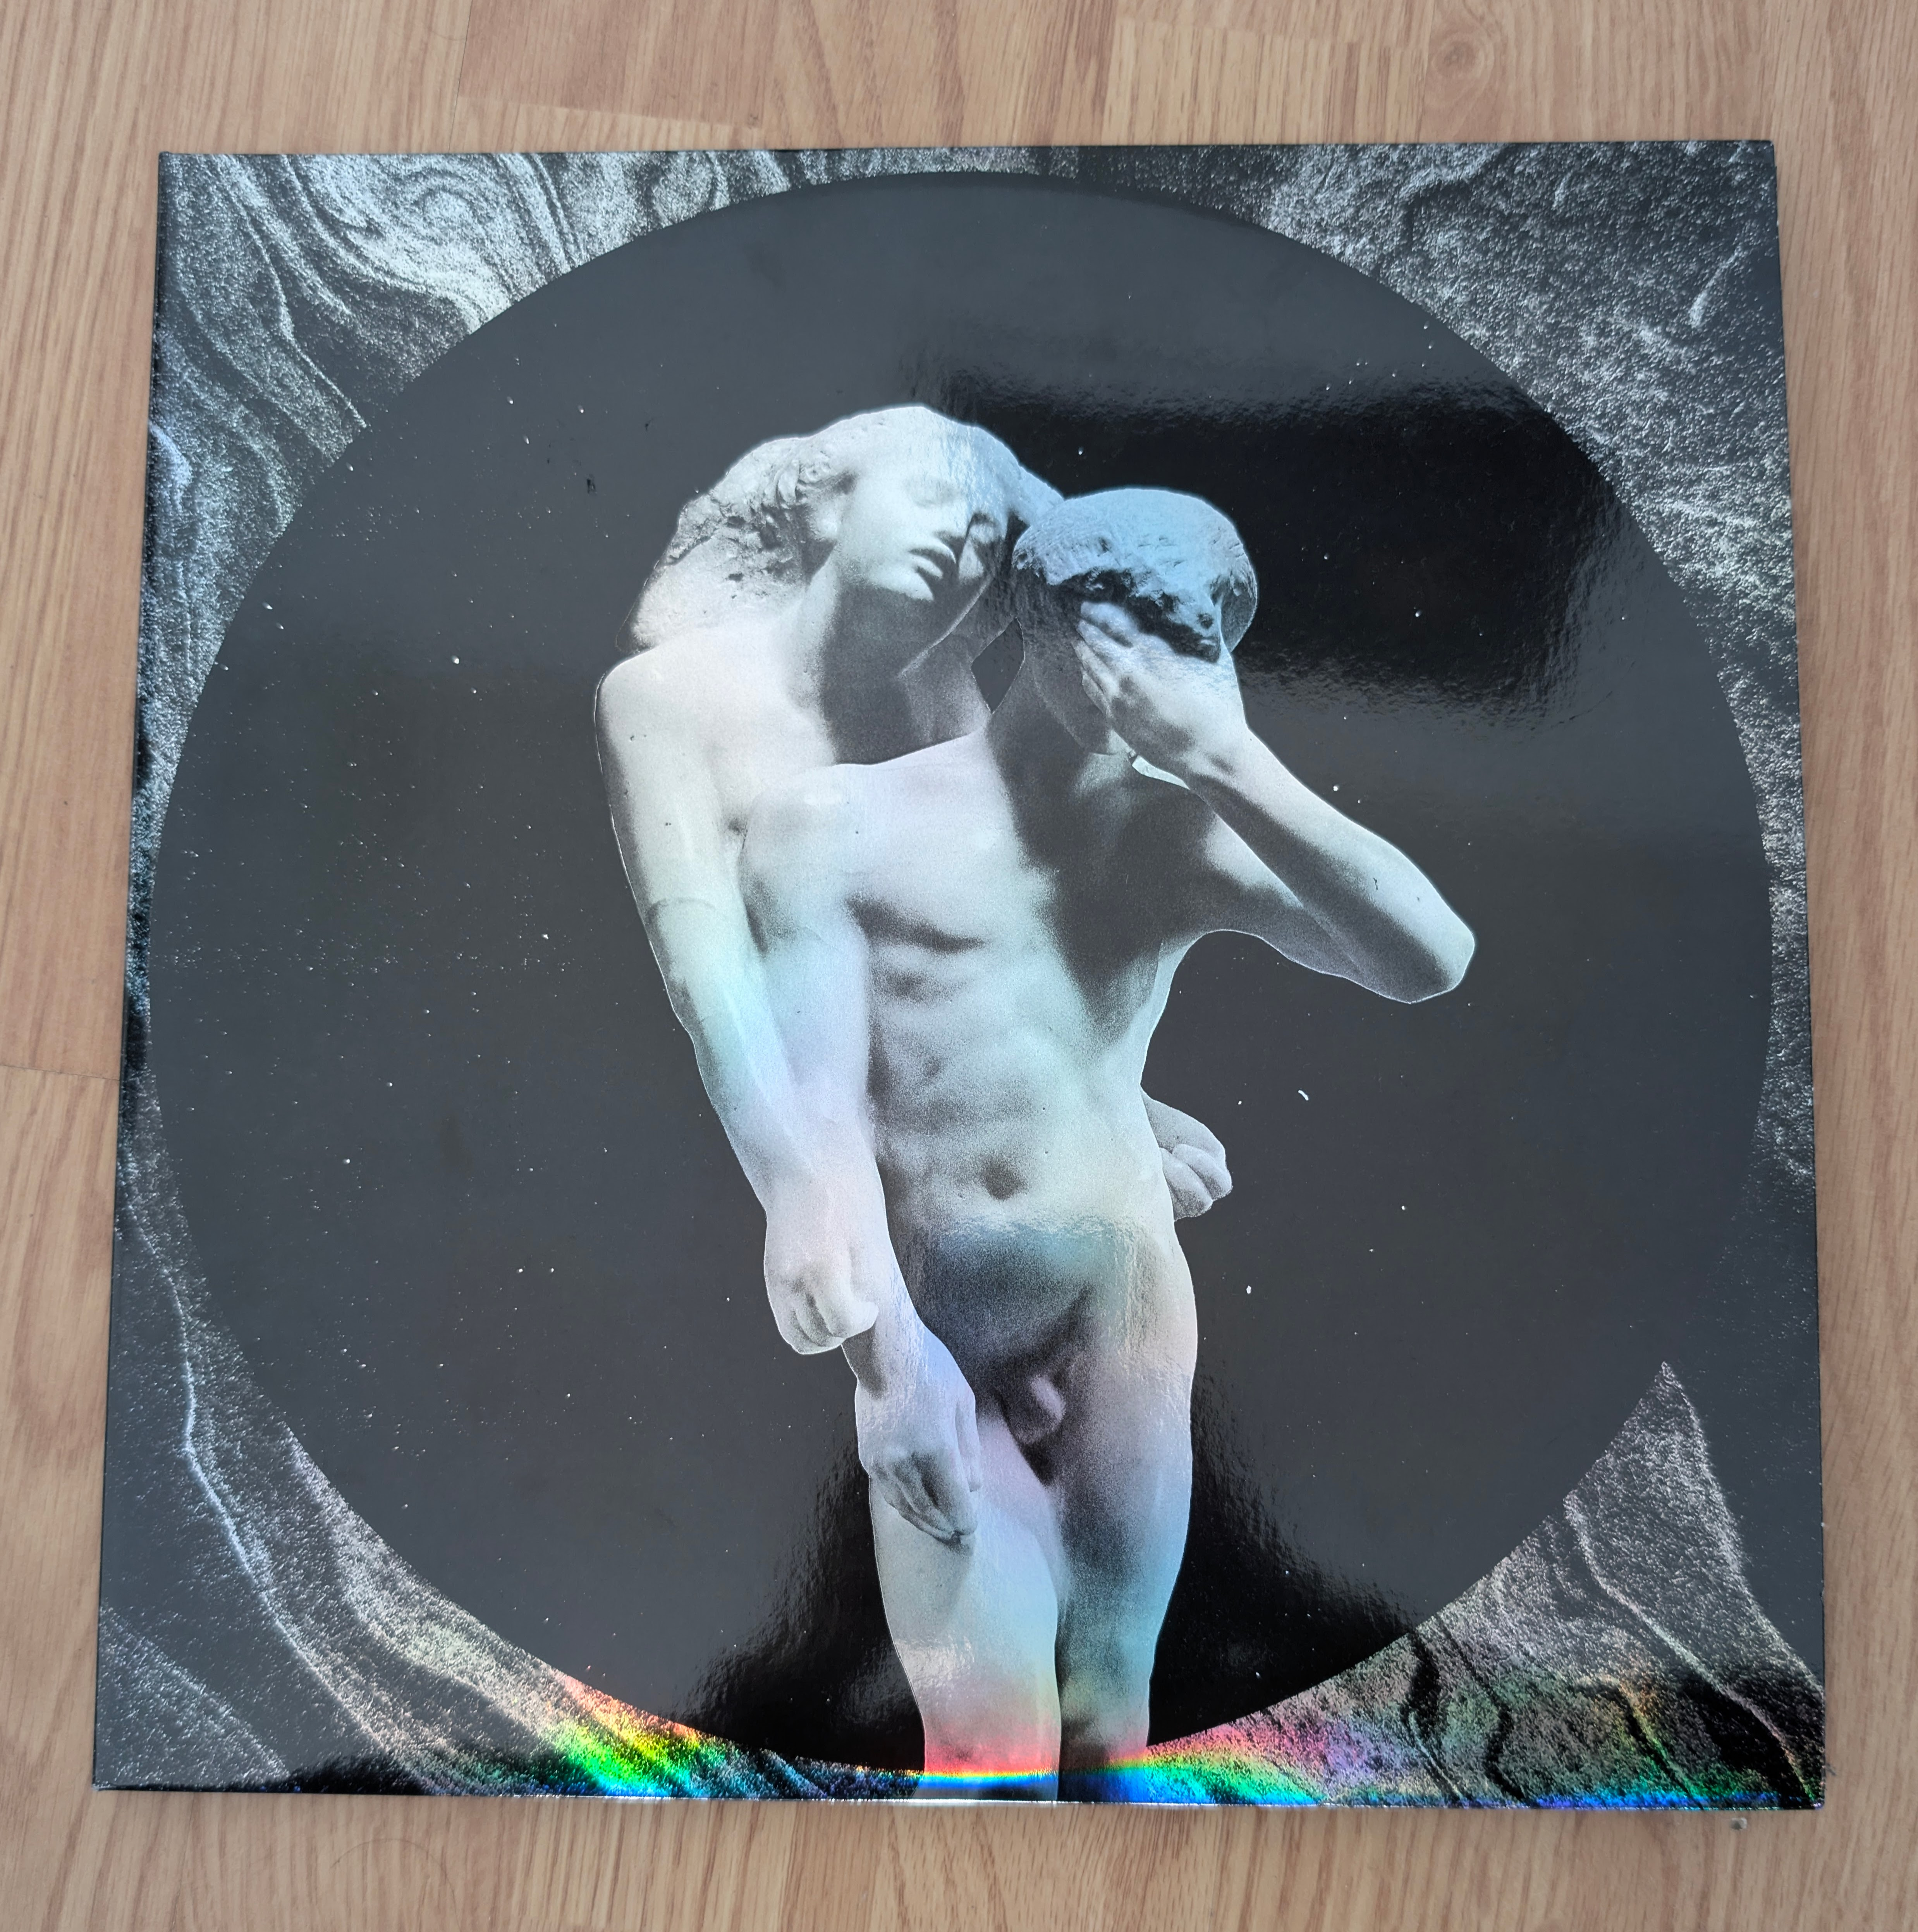
\includegraphics[width=2.5cm]{figures/test_albums/Reflektor.jpg} \\
            \hline
            Rotated $90$\textdegree & 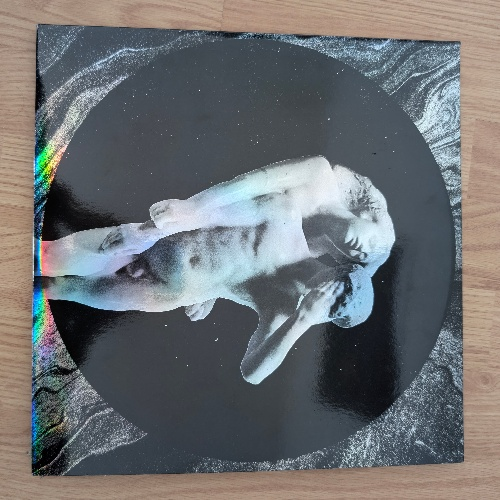
\includegraphics[width=2.5cm]{figures/test_albums/Reflektor_Rotated - 90.jpg} \\
            \hline
            Rotated $180$\textdegree & 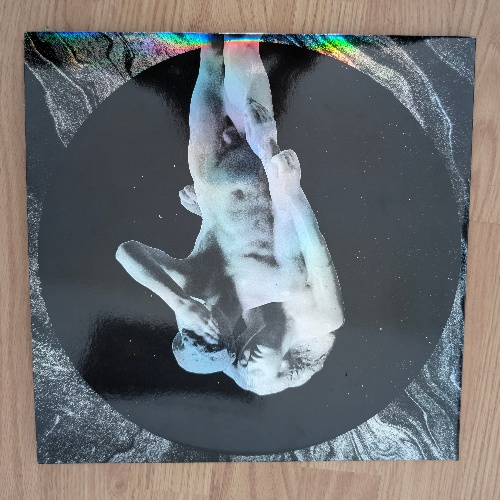
\includegraphics[width=2.5cm]{figures/test_albums/Reflektor_Rotated - 180.jpg} \\
            \hline
        \end{tabular}
    \end{subtable}
    \hfill
    \begin{subtable}{0.48\textwidth}
        \centering
        \begin{tabular}{|m{2.5cm}|m{2.5cm}|}
            \hline
            \textbf{Image Type} & \textbf{Example} \\
            \hline
            Rotated $270$\textdegree & 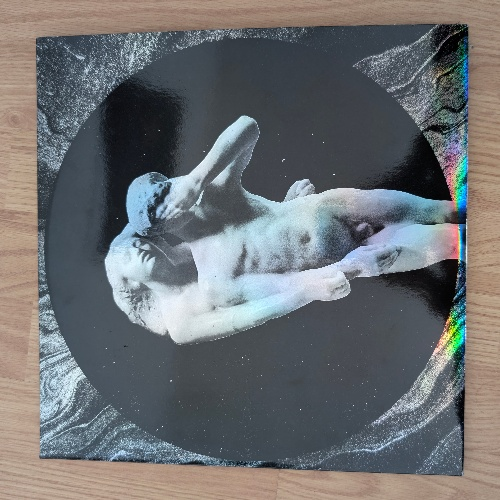
\includegraphics[width=2.5cm]{figures/test_albums/Reflektor_Rotated - 270.jpg} \\
            \hline
            Blurred & 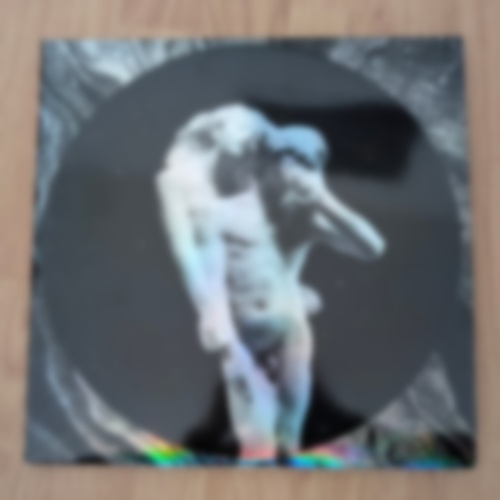
\includegraphics[width=2.5cm]{figures/test_albums/Reflektor_Blurred.jpg} \\
            \hline
            Scaled Down & 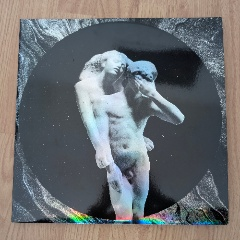
\includegraphics[width=2.5cm]{figures/test_albums/Reflektor_Scaled.jpg} \\
            \hline
        \end{tabular}
    \end{subtable}

    \caption{Example images used in the evaluation}
    \label{tab:image-evaluation-examples}
\end{table}

Self-taken images were preferred to ensure that the test cases were more representative of authentic user-uploaded images. This is opposed to using images already present on the Internet, which could be pre-indexed by search engines.

The criteria for a pass were defined as follows:
\begin{itemize}
    \item For reverse image search, a result was considered correct if the exact album name appeared in the returned results.
    \item For the Spotify search, a result was deemed correct if the correct album was returned.
\end{itemize}

\subsubsection{Results}
The results are split into two sets:
\begin{itemize}
    \item Reverse Image Search Accuracy – Displayed in Figure~\ref{fig:album-scanning-results-ris}, this dataset evaluates the accuracy of the Google Reverse Image Search API. While this API functions as a black box, as the application cannot affect its inner workings, evaluating its accuracy in practice is still valuable.
    \item Spotify Search Accuracy – Displayed in Figure~\ref{fig:album-scanning-results-spotify}, this dataset evaluates the accuracy of the Spotify Search API, considering only cases where the reverse image search correctly identified the album so the accuracy of the Spotify search could be isolated from the accuracy of the reverse image search.
\end{itemize}

\begin{figure} [H]
    \centering
    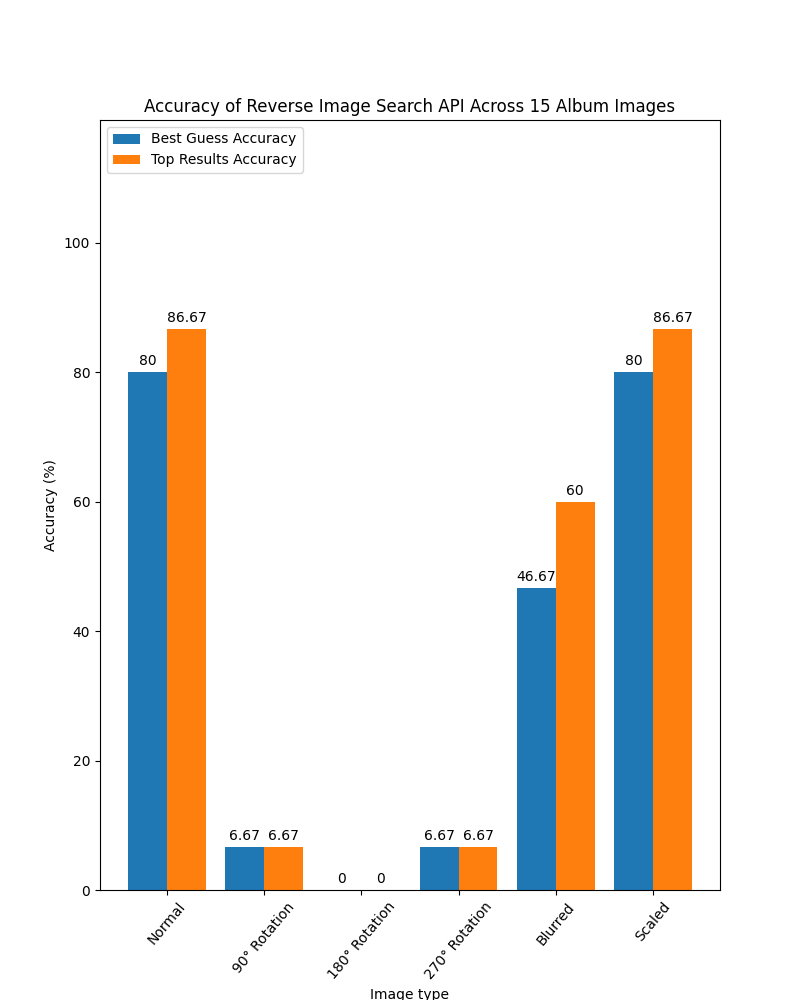
\includegraphics[width=0.65\textwidth]{figures/evaluation_graphs_ris.png}
    \caption{Accuracy of Reverse Image Search}
    \label{fig:album-scanning-results-ris}
\end{figure}

The results from the reverse image search did not meet expectations. While an accuracy of $95\%$ was targeted, the measured accuracy for images with no modification was significantly lower:
\begin{itemize}
    \item $80\%$ ($12$ out of $15$) accuracy when using the best guess from the reverse image search results.
    \item $86.67\%$ ($13$ out of $15$) accuracy when using website titles extracted from the search results.
\end{itemize}

Performance was particularly poor for rotated images, with only albums that had rotated artwork being correctly identified. The two examples of this in the test dataset are shown in Figures~\ref{fig:sos_rotated_90} and~\ref{fig:tih_rotated_270}.

\begin{figure} [H]
    \captionsetup{justification=centering}
    \centering
    \begin{subfigure}[t]{0.45\textwidth}
        \centering
        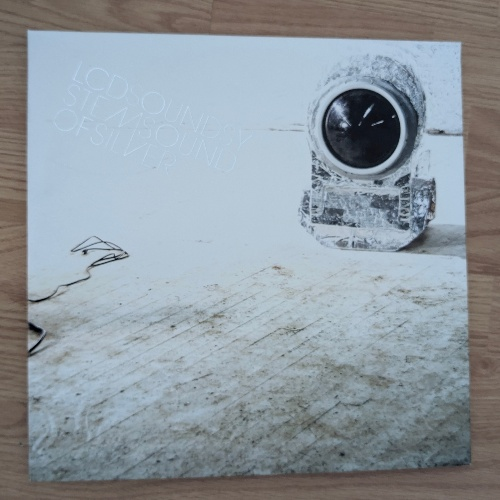
\includegraphics[width=0.45\textwidth]{figures/test_albums/Sound_Of_Silver_Rotated - 90.jpg}
        \caption{The only correct result for 90° rotation}
        \label{fig:sos_rotated_90}
    \end{subfigure}
    \begin{subfigure}[t]{0.45\textwidth}
        \centering
        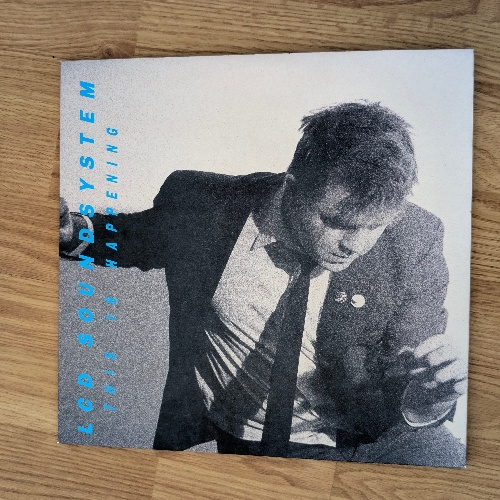
\includegraphics[width=0.45\textwidth]{figures/test_albums/This_Is_Happening_Rotated - 270.jpg}
        \caption{The only correct result for 270° rotation}
        \label{fig:tih_rotated_270}
    \end{subfigure}
\end{figure}

Despite the shortcomings of the reverse image search, the results indicate that the scatter-shot approach, using website titles, was equally or more successful across all categories of images. These results validate including it as it improves the overall chances of identification.

\begin{figure} [H]
    \centering
    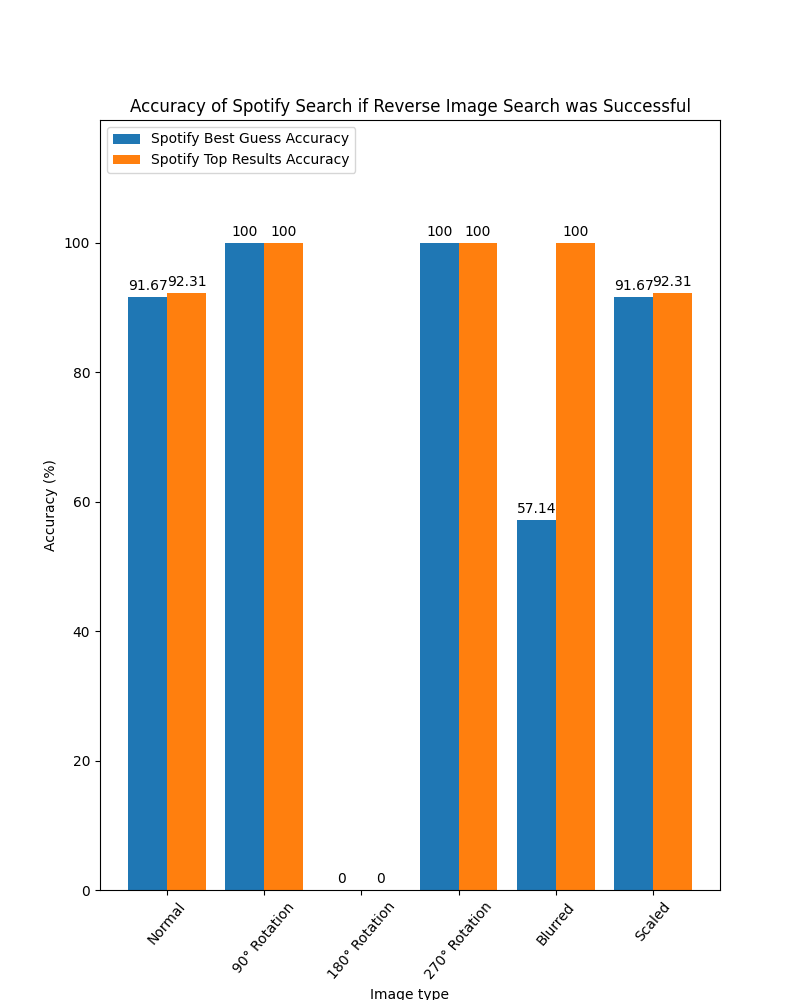
\includegraphics[width=0.65\textwidth]{figures/evaluation_graphs_spotify.png}
    \caption{Accuracy of Spotify Search}
    \label{fig:album-scanning-results-spotify}
\end{figure}

The results from the Spotify search API demonstrated strong performance. When provided with a correct reverse image search result, the Spotify search successfully identified the correct album in:

\begin{itemize}
    \item $91.67\%$ (11 out of 12 cases) for best guess searches.
    \item $92.31\%$ (12 out of 13 cases) for website title-based searches.
\end{itemize}

These results indicate that the chosen method, directly using reverse image search outputs with no processing as inputs for the Spotify search API, was broadly effective, even though it did not achieve the target $95\%$ accuracy.

\subsubsection{Key Takeaways}
The primary limiting factor in the system's accuracy is the reverse image search API's accuracy. Therefore, any changes hoping to improve the accuracy of album identification should focus on enhancing this API's accuracy.

Since the Google reverse image search API is treated as a black box, direct improvements to its internal processing are impossible, leaving only one option to improve its accuracy: input refinement. Two possible approaches include:

\begin{itemize}
    \item Pre-processing the image – Applying pre-processing techniques to remove backgrounds before passing the image to the API, for example, segmentation, where the image's background is removed automatically. %[TODO: Add a reference to segmentation potentially]
    \item User-assisted cropping – Prompting users to crop the image manually, ensuring only the album cover is submitted for identification
\end{itemize}

Though these methods may improve accuracy, the second could introduce additional UI elements, making the system more complex from a user perspective. The first may increase the time required to scan an album. Therefore, any enhancements should be carefully evaluated to balance accuracy improvements with user experience.

It should also be noted that the sample size for testing was relatively small, with only fifteen albums evaluated. As a result, the accuracy figures obtained may not fully represent the system's performance on a more extensive and diverse dataset. For example, less popular albums are likely less likely to be identified, and more popular albums are more likely to be identified. Testing with a broader selection of albums would be necessary to obtain a more comprehensive assessment of the system's accuracy and limitations.

\subsection{Album Playback}
This test aimed to verify that the music playback functionality operated as intended. The most effective approach was to evaluate the application from a user perspective, simulating real-world usage by using it to listen to whole albums, ensuring that playback functioned correctly.
\ifshowappendix
%Testing was conducted using a subset of five albums listed in Appendix~\ref{apd:test_albums}.
\fi

\subsubsection{Results}
The results of this test were entirely positive. All selected albums played from start to finish without issues. Additionally, the music controls, including play, pause, and skip—functioned as expected, and album artwork and track information were displayed correctly throughout playback as the tracks changed.

\section{User Interface}
The survey described in Section~\ref{sec:test-design} was used to evaluate the user interface. In total, seven participants completed the survey. Initially, the first user was given the application and asked to play around with it but based on their feedback the process was adjusted. Instead, users were given a list of objectives to complete to cover all functionality.

\subsection{Results}
\begin{table} [H]
    \centering
    \begin{tabular}{|m{5cm}|m{2cm}|m{2cm}|m{2cm}|}
        \hline
        \textbf{Question} & \textbf{Average} & \textbf{Minimum} & \textbf{Maximum} \\
        \hline
 How easy was the application to use? & $5.71$ & $3$ & $7$ \\
        \hline
 How visually appealing was the application? & $8.29$ & $6$ & $10$ \\
        \hline
 How useful did you find the ability to save albums to your collection? & $7.71$ & $5$ & $10$ \\
        \hline
 How valuable did/would you find the social features? & $5$ & $3$ & $8$ \\
        \hline
    \end{tabular}
    \caption{User Interface Evaluation Results}
    \label{tab:ui-evaluation-results}
\end{table}

The results for the first four questions in the survey are shown in Table~\ref{tab:ui-evaluation-results}.

\paragraph{Question 1: How easy was the application to use?}
In terms of usability, the application did not perform well. The average score was only $5.71$, suggesting most users struggled with the application at some point. This was most likely a result of the design of the interface. Some users added that certain features were hidden from them or not in the place they expected them to be. The example most frequently given was that the share collection buttons were not on the social page where they would make sense to be. One user also found they could not use the web browser of their choice as the application would appear broken. This was missed in testing as the developer only tested in Google Chrome.

\paragraph{Question 2: How visually appealing was the application?}
The visual appeal of the application was rated particularly highly, with an average score of $8.29$, though, as will be discussed in Section~\ref{sec:ui-evaluation-participants}, this could be a result of many participants sharing a view of what a visually appealing looks like.

\paragraph{Questions 3 and 4: How useful did you find the ability to save albums to your collection? \& How valuable did/would you find the social features?}
The two features that were asked about had very different perceptions from users. Having a collection associated with their account was seen as a good feature, with an average score of $7.71$. The social features were not seen as much of a benefit, with an average score of $5$. Users likely did not see the value in social features in such a small application.

\paragraph{Extra Comments From Users}
As part of the evaluation, users could add extra comments. Most were about UI design choices. Many users found the application different from what they would expect, and some struggled to figure out what to do on specific screens. This was particularly a problem on the landing screen, where users did not feel prompted to log in to continue.

Other users found minor visual bugs that were not picked up in testing. Variation in screen sizes was the most common cause of these bugs. During development, the developer focused on a single screen size and resolution (16:9 aspect ratio). This also limited the application's usability, with one user commenting that the application might be more useful on a phone.

\subsection{Participants}~\label{sec:ui-evaluation-participants}
Ideally, the user interface evaluation would have been conducted with a large and diverse user base to gather feedback from individuals with varying levels of technical expertise. However, this was beyond the scope of the current evaluation, so a smaller sample group was used instead.

It is important to acknowledge the potential biases in the participant selection. The sample group consisted primarily of friends and family, many of whom were computer science students. As a result, the participants may have been more familiar with the technology than the average user. They could also have been predisposed to providing more favourable reviews as to not disappoint the application's developer. Because of this, while the survey provides valuable insights, the findings may not fully represent a broader user base.

\section{Development Practices}
The development practices were evaluated based on the tests in Section~\ref{sec:test-design}. A pass was defined as meeting the verification specified.

\subsection{Testing And Test Coverage}
All tests defined in all test cases were executed and passed, as expected, as automated actions enforced this before code could be merged into the main branch of the repository.

Test coverage was measured using pytest-cov for the backend and Vitest for the frontend. The target was set at $95\%$ line and branch coverage for both the frontend and backend. The results are shown in Table~\ref{tab:test-coverage-results}.
\begin{table} [H]
    \centering
    \begin{tabular}{|m{3cm}|m{3cm}|}
        \hline
        \textbf{Component} & \textbf{Coverage} \\
        \hline
        Backend & $100\%$ \\
        \hline
        Frontend & $95\%$ \\
        \hline
    \end{tabular}
    \caption{Test Coverage Results}
    \label{tab:test-coverage-results}
\end{table}

The backend achieved full coverage with all lines and branches tested. The frontend achieved $95\%$ coverage, which whilst meeting the target, the fact it was below $100\%$ is likely a result of the inexperience of the developer in frontend development with many changes needed even after the tests were originally defined.

However, as was seen in the user evaluation of the interface, the tests did not manage to catch all minor issues suggesting the automated tests were either not comprehensive enough or secondary measures needed to be taken to ensure the application was fully functional.

In terms of the initial criteria set out in Section~\ref{sec:test-design}, the result was a success. But in terms of producing a fully functional, bug free application, the tests alone were not enough suggesting the initial criteria were not stringent enough.

\ifshowappendix
%A complete list of the tests can be found in Appendix~\ref{apd:testcases}.
\fi

\subsection{Code Quality}
Using pre-commit hooks successfully achieved the code quality objectives of enforcing formatting and linting. This ensured that all code committed to the repository adhered to established formatting and linting rules.

Though this approach was practical for a single developer, in hindsight, it may not have been ideal for team-based development because pre-commit hooks require each developer to install them manually. A much more robust approach would have been to enforce these rules using GitHub Actions that run on pull requests. This could either format the code itself or reject the pull request if the code did not meet the required standards, forcing the developer to run the formatting and linting tools locally before pushing their changes, achieving the same goal as the pre-commit hooks.

\subsection{Automated Deployment and Dependency Management}
The automated deployment process was successfully implemented. Once configured on Google Cloud Run, the application could be rebuilt and deployed automatically whenever a new tag was pushed to the repository.

Similarly, automated dependency management was effectively set up using Dependabot, with weekly checks for updates. Throughout development, $110$ pull requests were generated for dependency updates, with only three requiring manual intervention, primarily due to breaking changes. It is of note that none of the changes that passed all tests resulted in breaking changes to the application, suggesting that the testing system in place was effective in verifying functionality after each update.
